\section{B-tree}
        \textbf{В-дерево} - сильноветвящееся сбалансированное дерево поиска, позволяющее проводить поиск, добавление и удаление элементов за О log(m).
        \par
        Благодаря тому, что В-дерево сбалансированное и каждый элемент расположен сравнительно близко к корню, имеет высоту О log(m). Например, для поиска элемента, мы можем проверить средний элемент, если он больше искомого, то отбросим вторуб половину, если же меньше, то наоборот - отбросим начальную половину, и так будем продолжать делить пополам, в итоге проверим log(m) элементов.
        \par
         Некоторые сбалансированные деревья хранят значения только в конечных узлах. B-деревья хранят значения в каждом узле дерева. Каждый внутренний узел В-дерева содержит ключи, которые разделяют его поддеревья. Например. Если узел имеет 3 потомка, то он должен иметь 2 ключа k1, k2. Все значения в крайнем левом поддереве меньше k1, в среднем поддереве они будут между k1 и k2, а в крайнем правом – больше, чем k2.
         \par
         В отличие от остальных деревьев, они созданы специально для эффективной работы с дисковой памятью, они минимизируют обращения типа ввода-вывода. Это происходит благодаря тому, что в одном узле можно хранить много ключей и при этом можно ссылаться на несколько дочерних узлов. Значительно уменьшив высоту дерева, увеличивается доступ к диску. 
         \par
        В-дерево порядка m – это дерево, удовлетворяющее следующим свойствам:
        \begin{enumerate}
    \item Все листья находятся на одном уровне, т. е. обладают одинаковой глубиной, равной высоте дерева. 
    \item Ключи в каждом узле упорядочены по возрастанию
    \item Каждый узел может иметь максимум m потомков
    \item Каждый узел может содержать максимум (m-1) ключей
    \item У каждого узла должно быть минимум (m/2) потомков
    \item Узел, кроме корня, должен содержать минимум ([m/2]-1) ключей
\end{enumerate}
        
        На рисунке изображено дерево порядка 4, удовлетворяющее этим свойствам:\par
        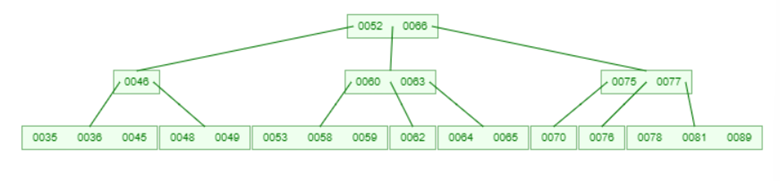
\includegraphics[width=1\linewidth]{tree_ex.png} \par
        \newpage
        \subsection{Операции}
        B-деревья представляют собой сбалансированные деревья, поэтому время выполнения стандартных операций в них пропорционально высоте. Однако, как уже было упомянуто выше, алгоритмы B-дерева созданы специально для работы с дисками (или другими носителями информации) и базами данных (или иными видами представления большого количества информация), минимизируя количество операций ввода-вывода. \par
        \textbf{Виды:} \par
        \begin{enumerate}
    
    \item Поиск
    \item Вставка
    \item Удаление

\end{enumerate}
    
        \subsection{Поиск по B-tree}
        В В-дереве поиск начинается с корневого узла, но на каждом шаге принимается n-стороннее решение, где n – это общее количество потомков рассматриваемого узла. Поиск происходит следующим образом:\par
        \begin{enumerate}
    \item Начиная с корня, сравнивается k с первым ключом узла. Если k первый ключ в узле, то необходимо вернуть узел и индекс.
    \item Если k является листом, то вернуть NULL.
    \item Если k меньше первого ключа в корне, тогда рекурсивно искать левого потомка этого ключа.
    \item Если в текущем узле есть более одного ключа и k больше первого, сравнить k со следующим ключом в узле. Если k меньше следующего ключа, тогда ищем левого потомка. В противном случае выполняется поиск правильного дочернего элемента ключа. 
    \item Повторять с 1 по 4, пока не дойдем до листа.

\end{enumerate}
    

        \newpage
        \textbf{Пример:} \par
        1.	Будем искать k = 17 в В-дереве ниже степени 3. \par
        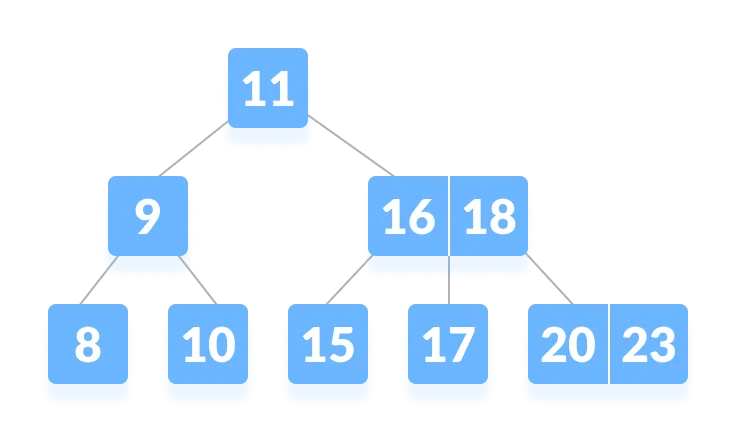
\includegraphics[width=0.6\linewidth]{search-1.jpg} \par
        2.	K не найден в корне, следовательно сравниваем его с корневым ключом \par
        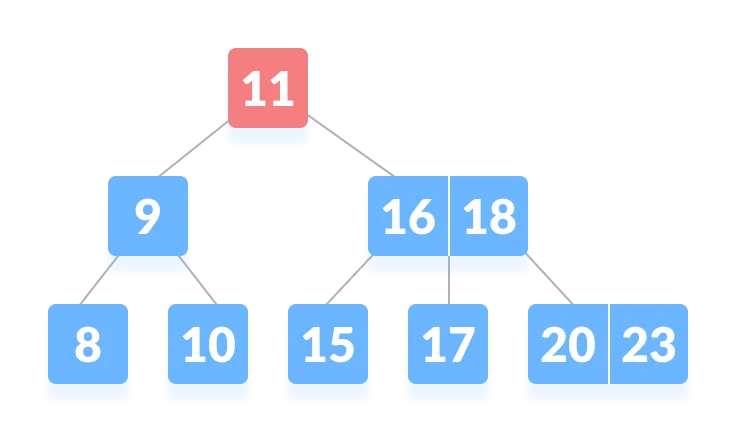
\includegraphics[width=0.6\linewidth]{search-2.jpg} \par
        3.	Так как k > 11, необходимо перейти к правому потомку \par
        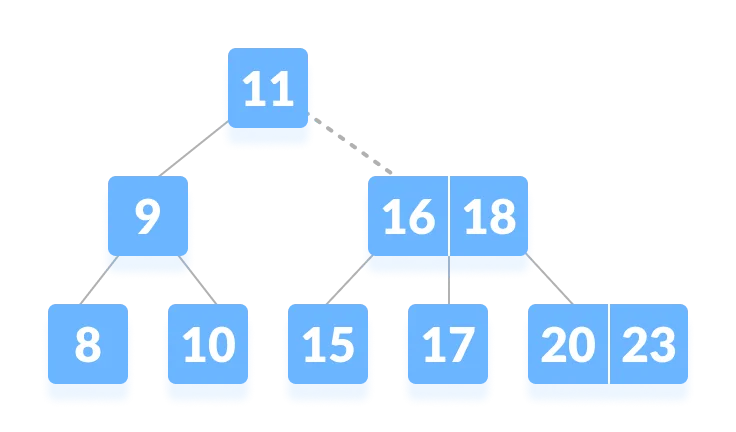
\includegraphics[width=0.6\linewidth]{search-3.jpg} \par
        \newpage
        4.	Сравниваем k с 16. Поскольку k>16Ю сравниваем k со следующим ключом 18 \par
        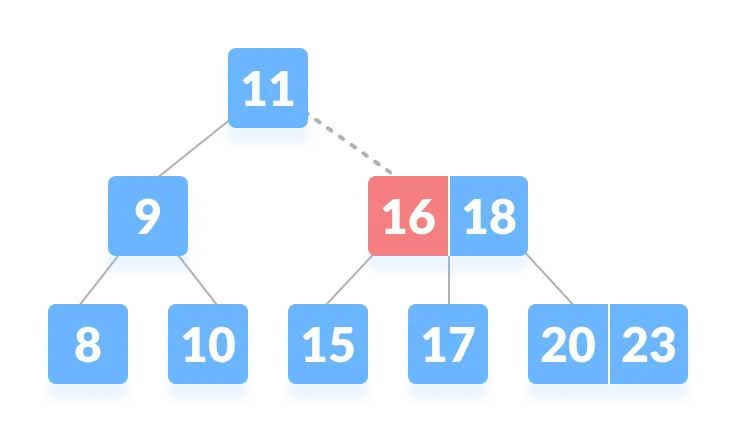
\includegraphics[width=0.6\linewidth]{search-4.jpg} \par
        5.	Поскольку k < 18, значит он находится между 16 и 18. Поиск происходит в правом или левом потомке. \par
        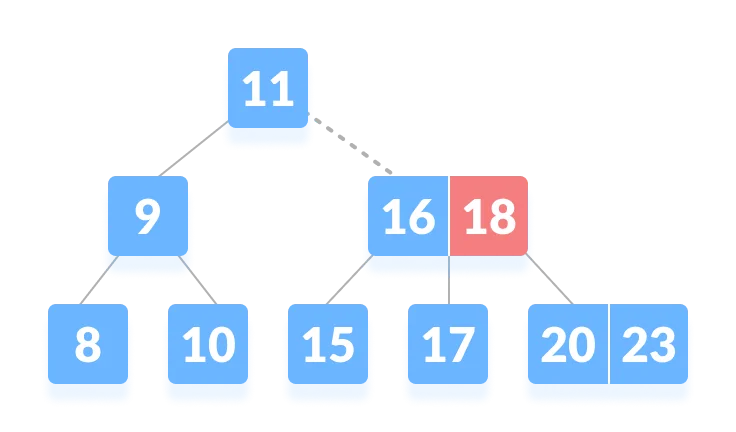
\includegraphics[width=0.6\linewidth]{search-5.jpg} \par
        6.	K найдено. \par
        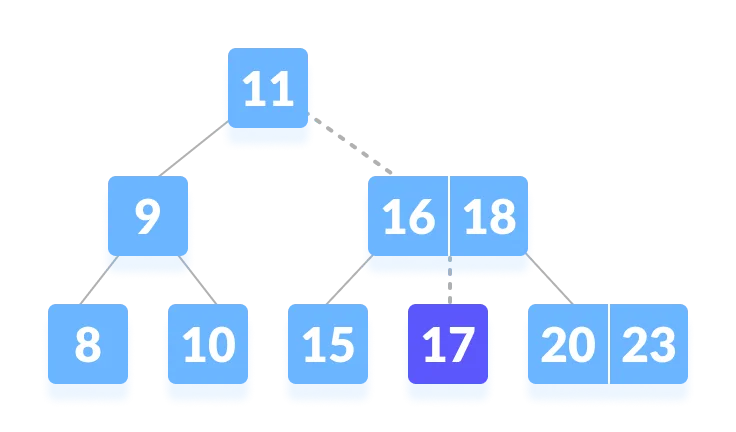
\includegraphics[width=0.6\linewidth]{search-6.jpg} \par
        \newpage
        \subsection{Вставка в B-tree} 
        Вставка элемента в В-дерево состоит из двух событий: поиска соответствующего узла для вставки элемента и разделения узла при необходимости. \par
        \begin{enumerate}
    \item Если дерево пусто, выделите корневой узел и вставьте ключ.
    \item Обновите допустимое количество ключей в узле.
    \item Найдите соответствующий узел для вставки.
    \item Если узел заполнен, вставьте элементы в порядке возрастания.
    \item Теперь есть элементы, превышающие его предел, необходимо разделить посередине.
    \item Переместите средний ключ вверх и сделайте левые ключи левыми дочерними, а правые – правыми дочерними.
    \item Если узел не заполнен, вставьте узел в порядке возрастания.
\end{enumerate}
        \textbf{Пример:} \par
        Вставляем элементы: 8, 9, 10, 11, 15, 20, 17. \par
        \begin{center}
            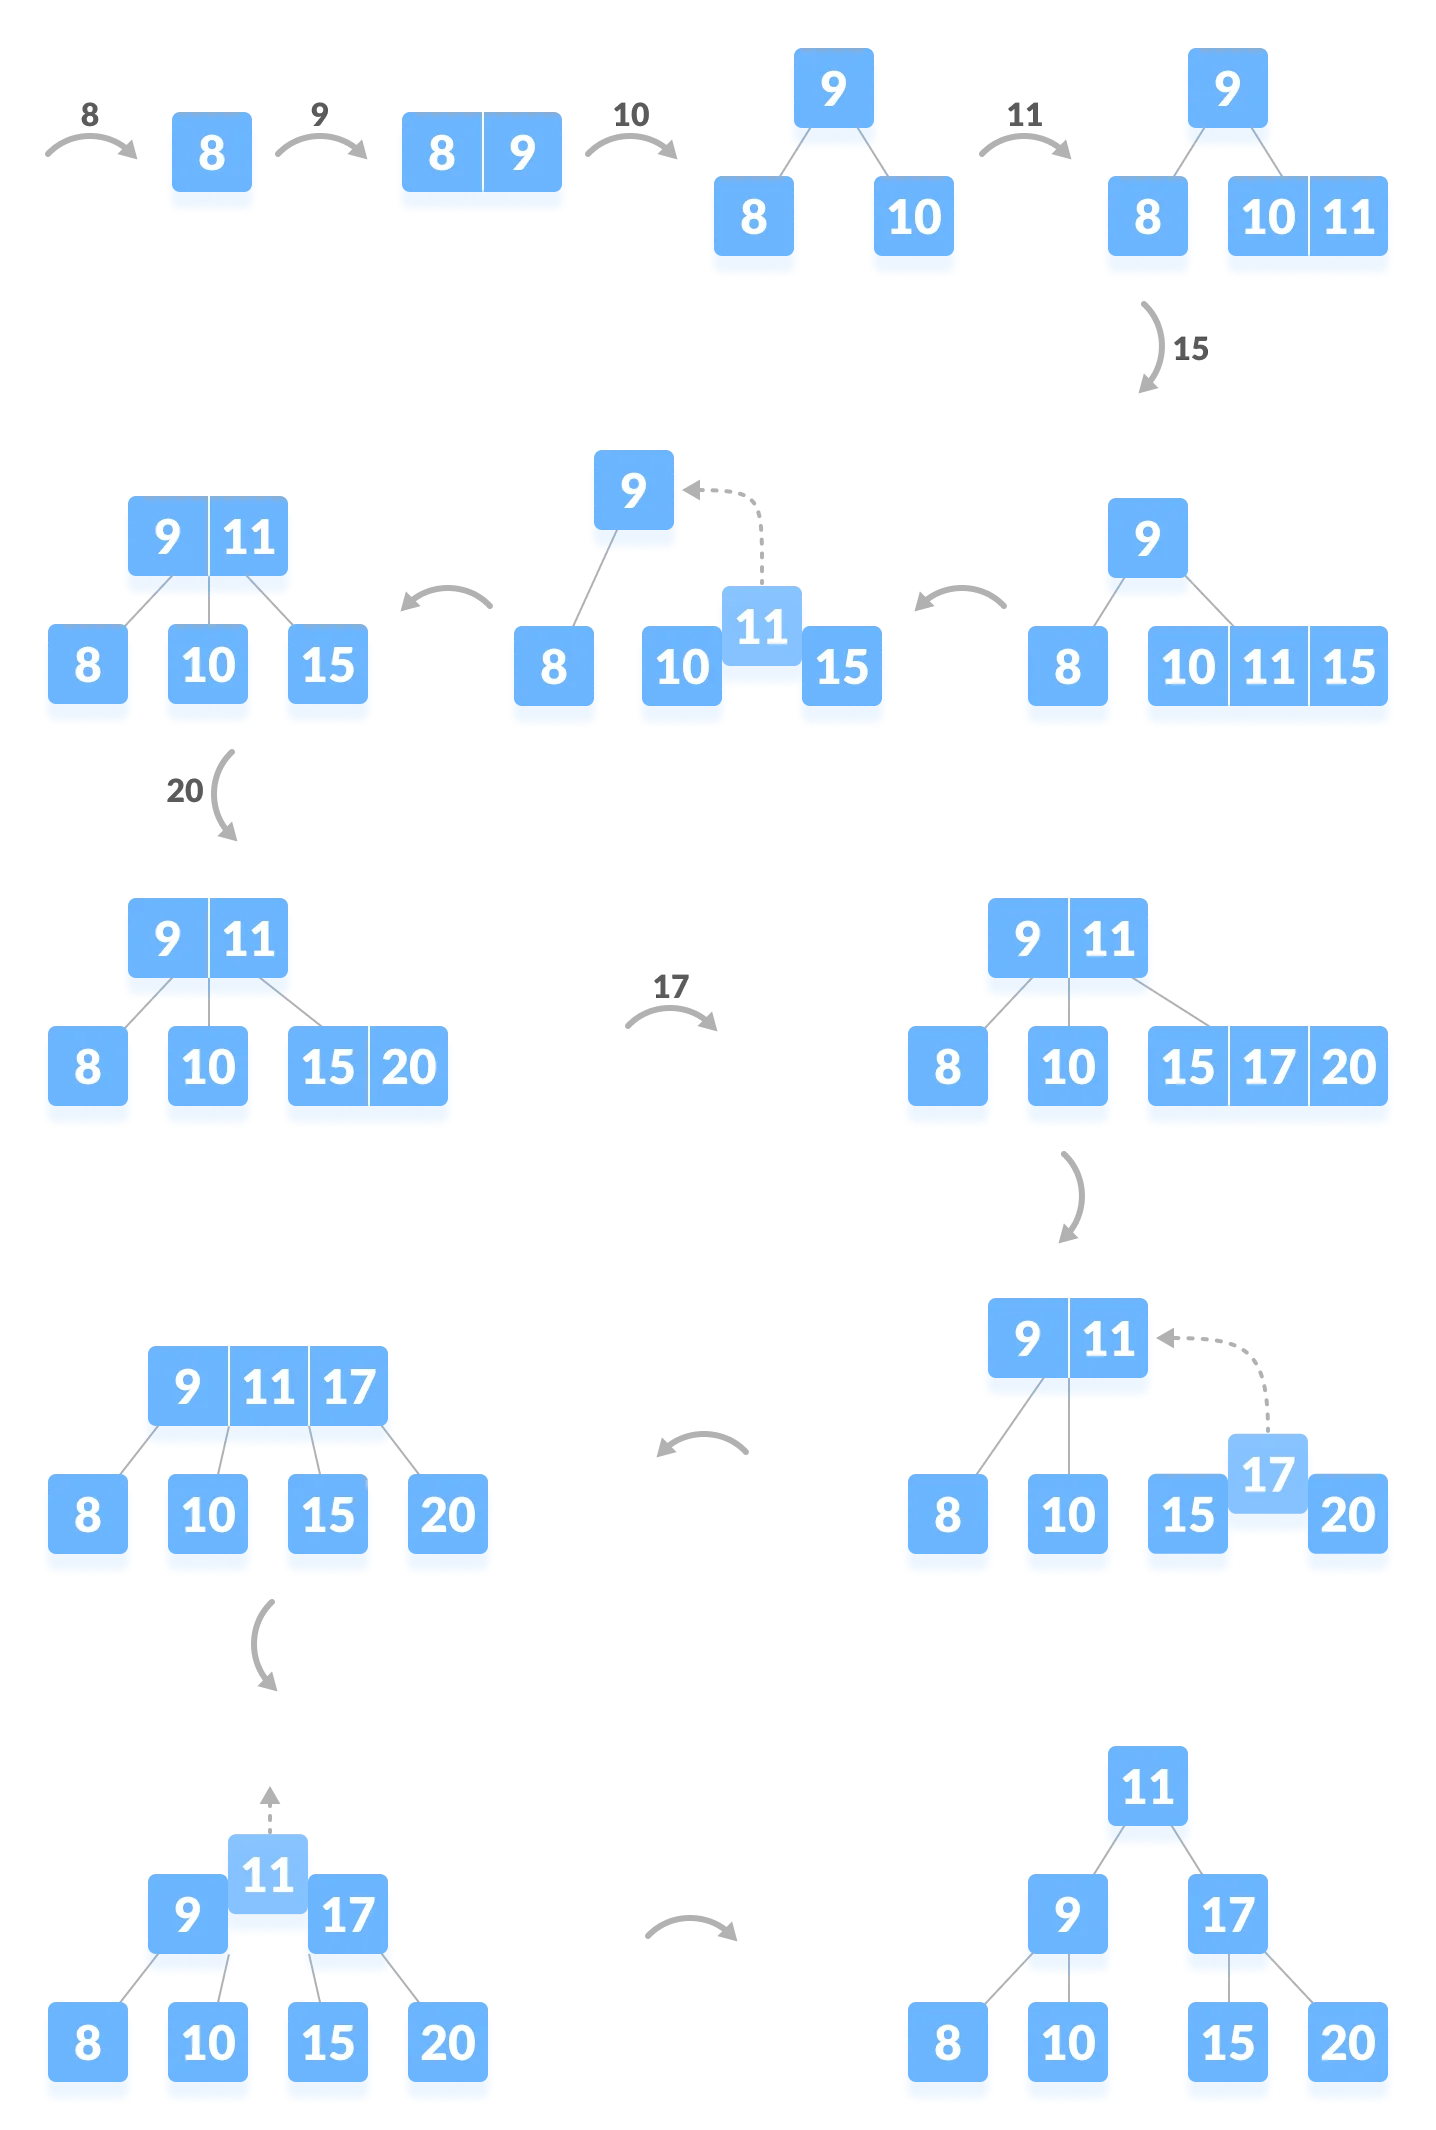
\includegraphics[width=0.45\linewidth]{insertion.jpg} \par
        \end{center}
        \newpage
        \subsection{Удаление из B-tree}
        Удаление состоит из трех основных событий: поиск узла, в котором существует удаляемый ключ; удаление ключа и при необходимости балансировка дерева. \par
        При удалении дерева может возникнуть состояние – недостаток памяти. Но дополнение происходит, когда узел содержит меньше минимального количество ключей, которое он должен содержать. \par
        Существует три основных случая при удалении в В-дереве. \par
        \textbf{Случай №1} \par
        Ключ, который нужно удалить, лежит в листе. Для этого есть два случая. \par
        \begin{enumerate}
            \item Удаление ключа не нарушит свойство минимального количества ключей, которое должен иметь узел. Пример: удаление 32 \par
            \begin{center}
                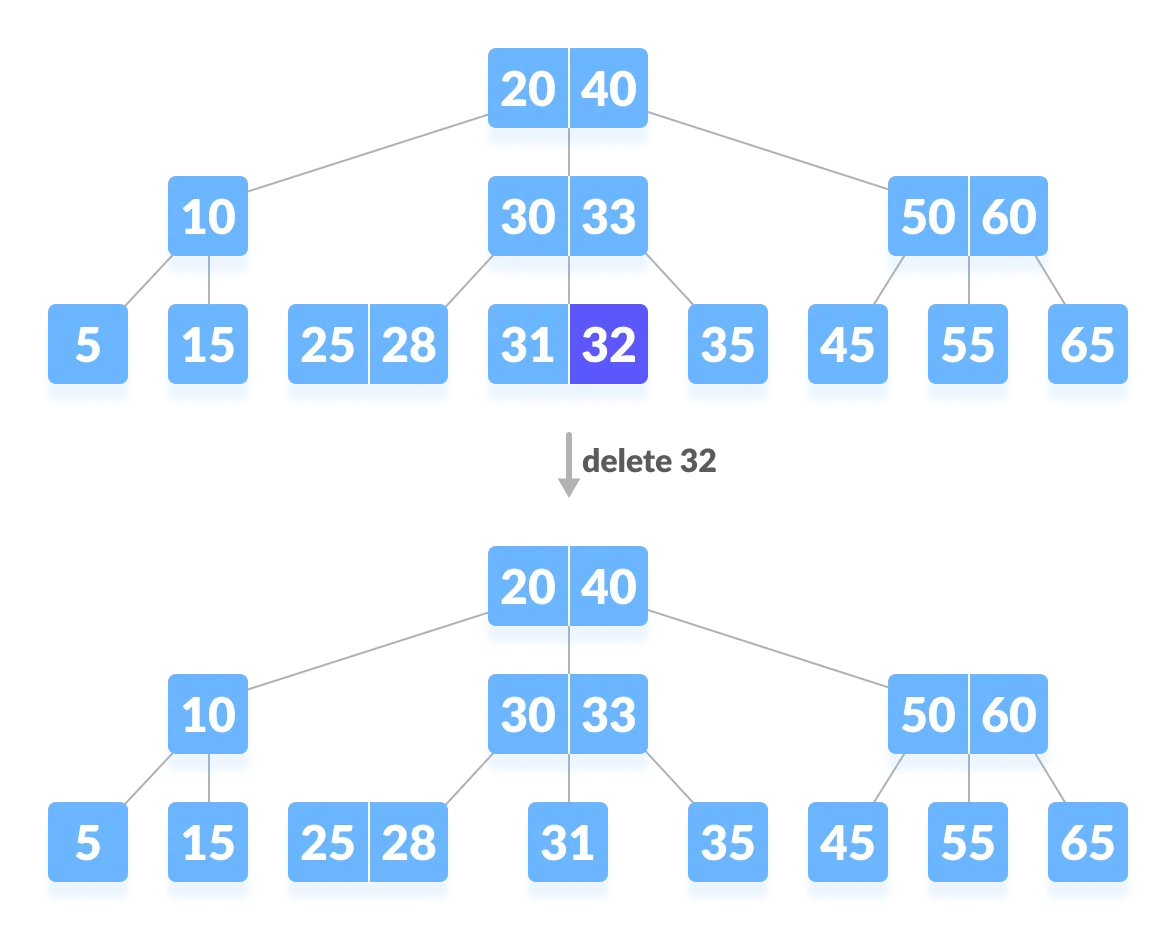
\includegraphics[width=0.8\linewidth]{удал.jpg} \par
            \end{center}
            \newpage
            \item Удаление ключа нарушает свойство минимального количества ключей. В этом случае мы заимствуем ключ у соседнего родственного узла в порядке слева направо.
            \begin{itemize}
                \item Перейти к ближайшему левому брату, если он имеет больше минимального количества ключей, то заимствуйте ключ из этого узла.
                \item Иначе, отметьте, чтобы заимствовать из правого родственного узла. В дереве ниже удаление 31 приводит к указанному выше условию, будем заимствовать ключ из левого узла.
            \end{itemize}
            \begin{center}
                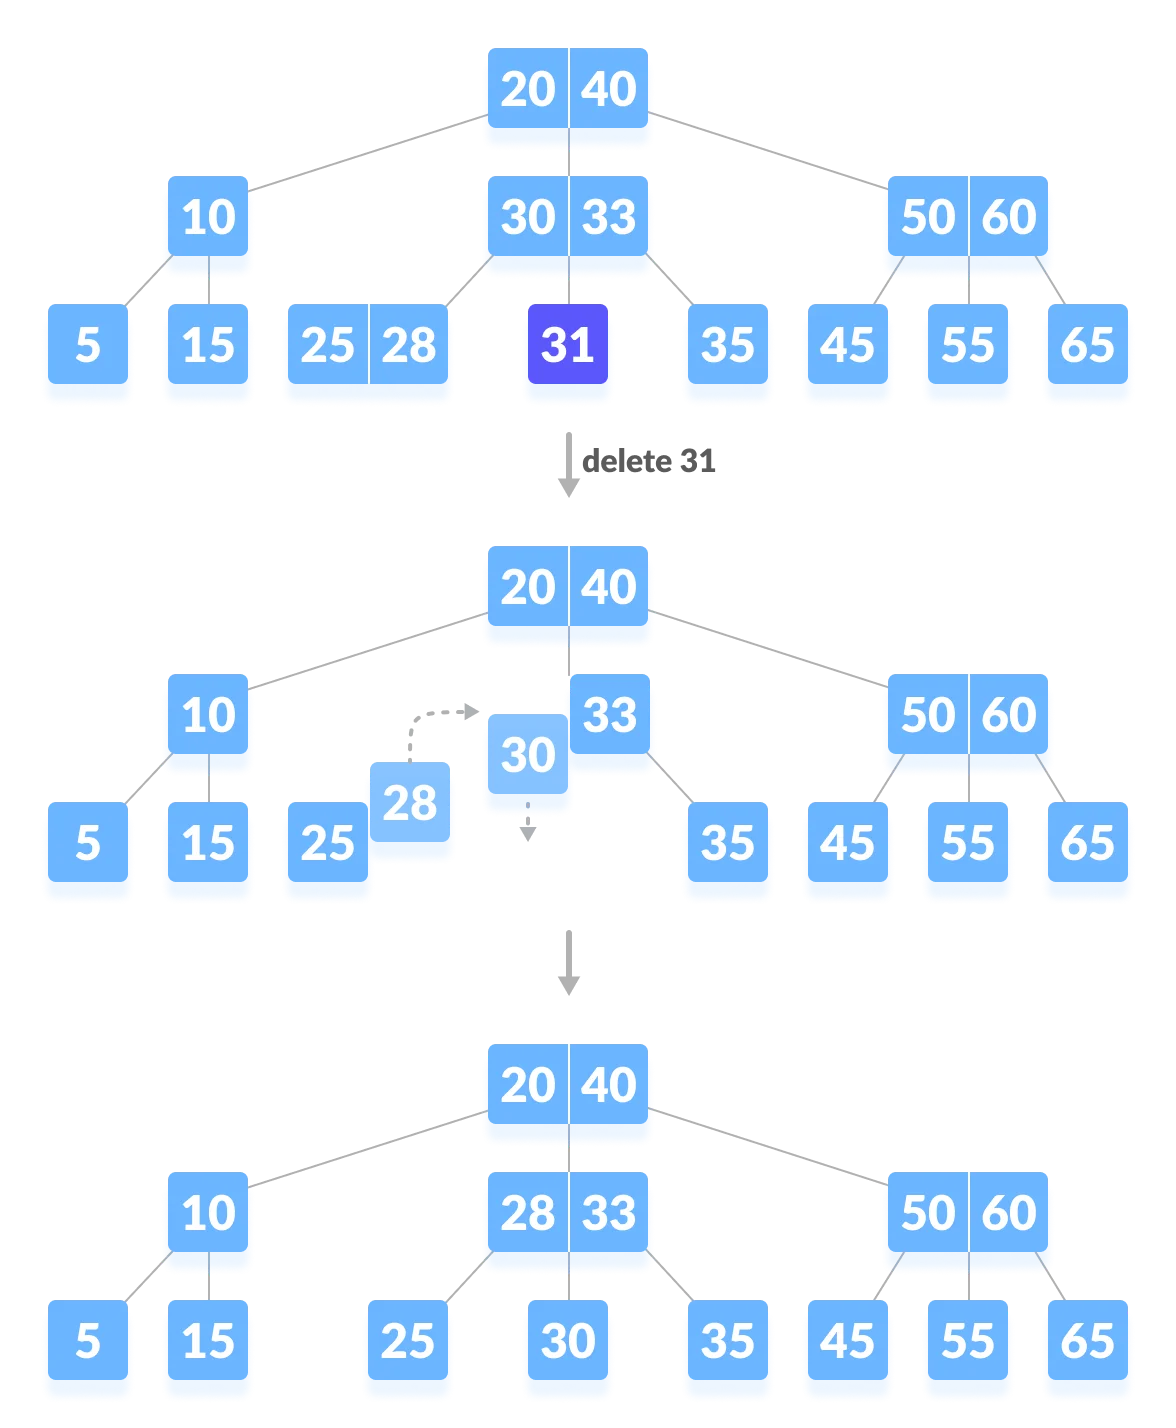
\includegraphics[width=0.8\linewidth]{удал2.jpg} \par
            \end{center}
            \newpage
            \item Если оба одноуровневых узла уже имеют минимальное количество ключей, то нужно объединить узел либо с левым, либо с правым узлом. Это слияние выполняется через родительский узел. \par
            \begin{center}
                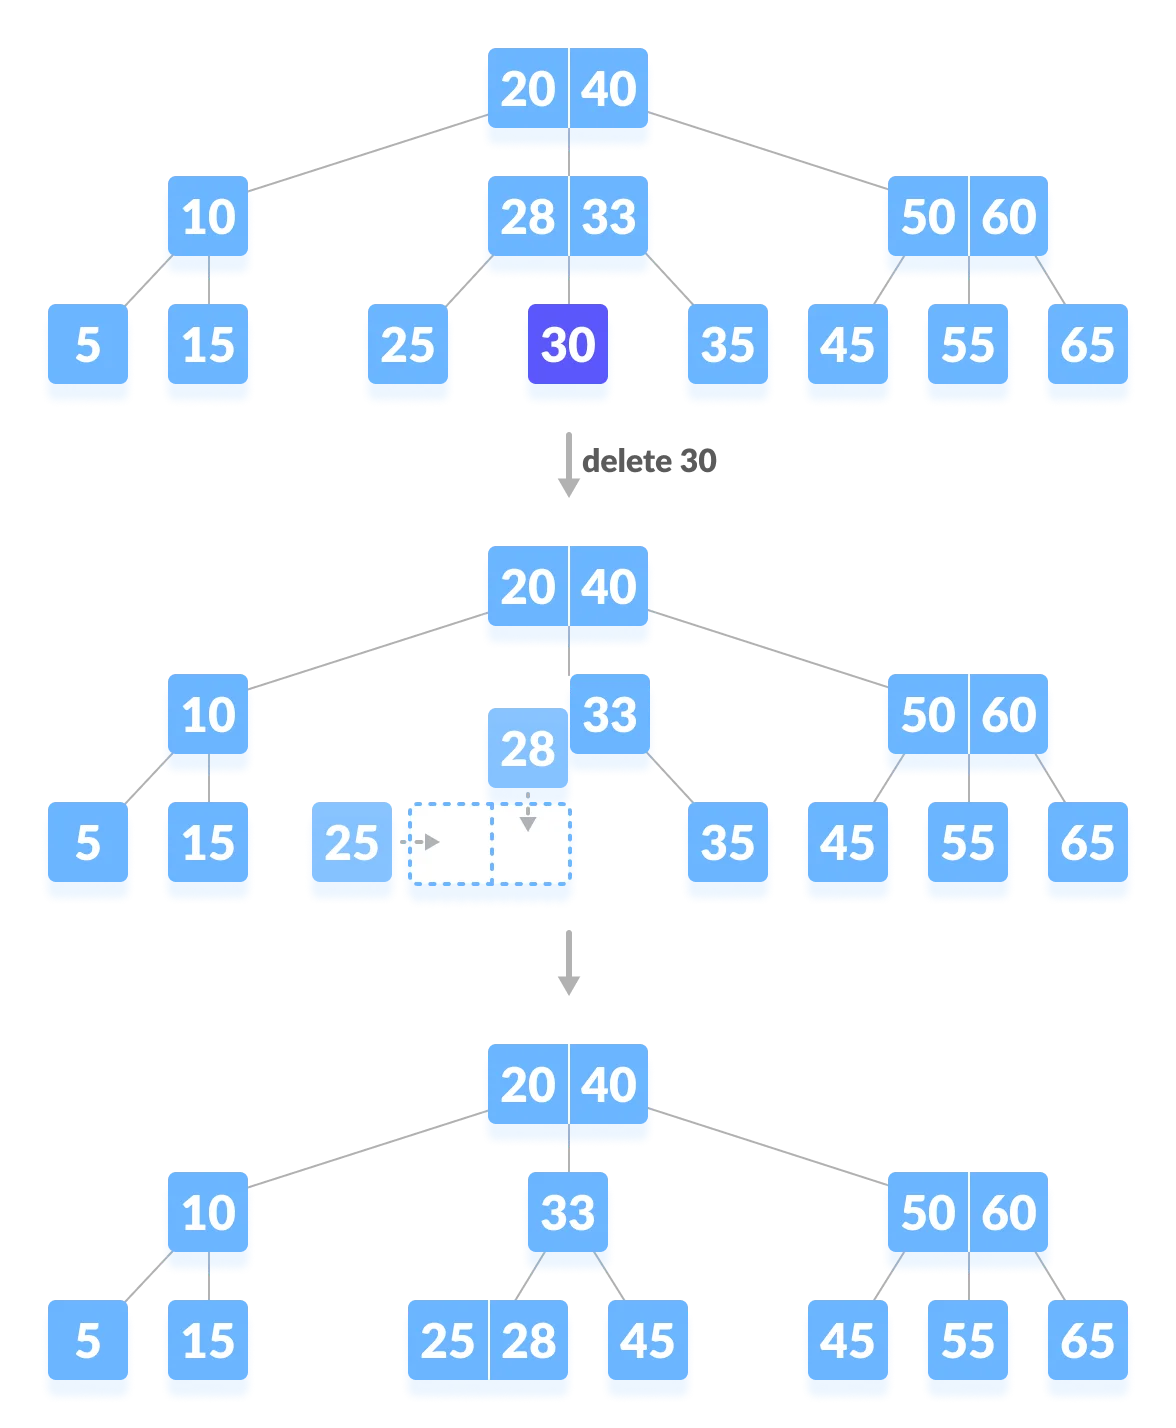
\includegraphics[width=0.8\linewidth]{удал 3.jpg} \par
            \end{center}
            \newpage
        \end{enumerate}
        \textbf{Случай №2} \par
        Если удаляемый ключ лежит во внутреннем узле, возникают следующие случаи: \par
        \begin{enumerate}
            \item Внутренний узел, который удаляется, заменяется неупорядоченным предшественником, если левый дочерний узел имеет больше минимального количества ключей.
            \begin{center}
                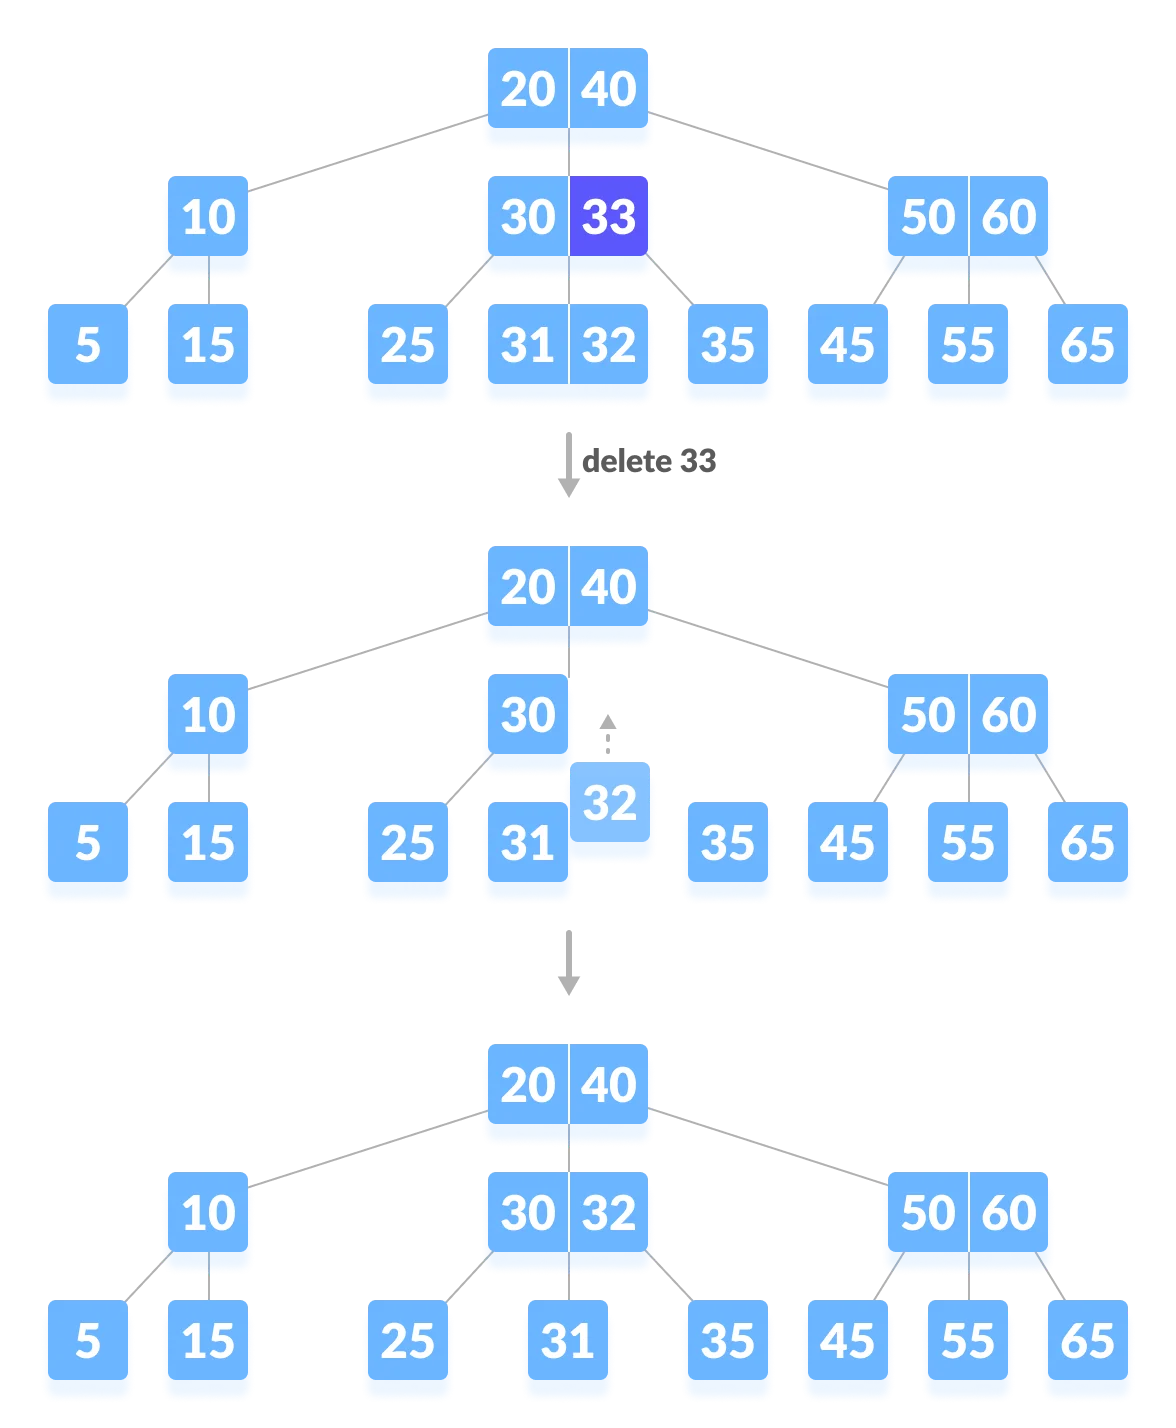
\includegraphics[width=0.8\linewidth]{удал 4.jpg} \par
            \end{center}
            \newpage
            \item Внутренний узел, который удаляется, заменяется преемником по порядку, если правильный дочерний узел имеет больше, чем минимальное количество ключей
            \item Если любой из дочерних элементов имеет точно минимальное количество ключей, объедините левый и правый дочерний элементы. После слияния, если родительский узел имеет меньше минимального количества ключей, ищите братьев и сестер, как в случае 1.
            \begin{center}
                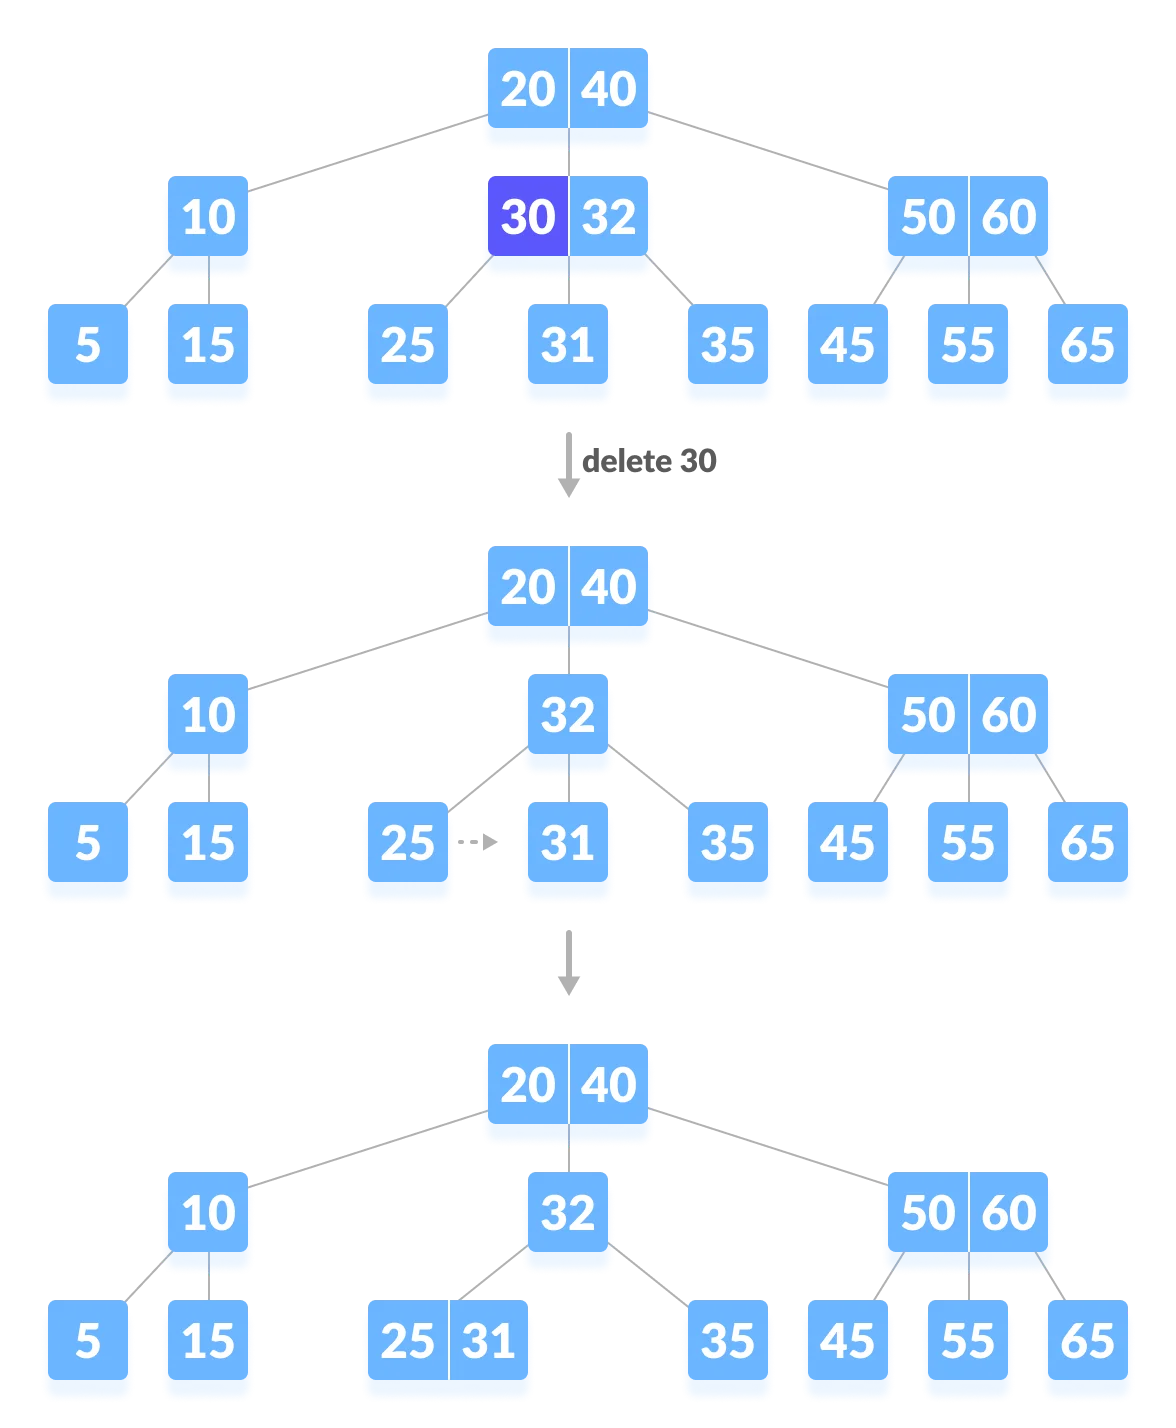
\includegraphics[width=0.8\linewidth]{удал 5.jpg} \par
            \end{center}
            \newpage
        \end{enumerate}
        \textbf{Случай №3} \par
        При этом высота дерева уменьшается. Если целевой ключ лежит вл внутреннем узле, а удаление ключа приводит к уменьшению числа ключей в узле (то есть меньше минимально необходимого), то ищите неупорядоченного преемника. Если оба дочерних элемента содержит минимальное количество ключей, то заимствование невозможно. Это приводит к слиянию дочерних элементов. \par
        \begin{center}
                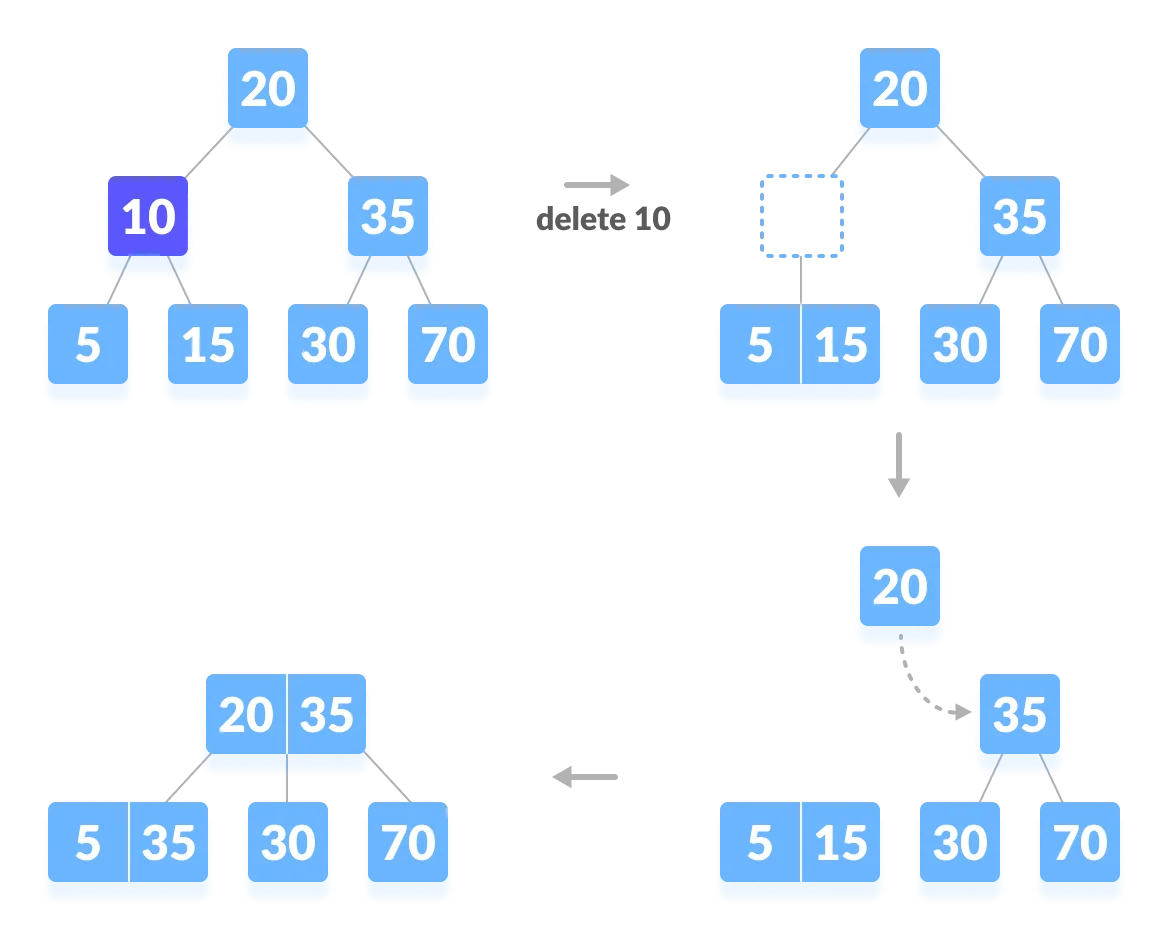
\includegraphics[width=1\linewidth]{удал п.jpg} \par
        \end{center}
        \newpage
        \textbf{Преимущества B-tree} \par
        \begin{itemize}
            \item Уменьшает количество операций чтения на диске 
            \item B Деревья могут быть легко оптимизированы для настройки их размера (то есть количества дочерних узлов) в соответствии с размером диска.
            \item Это специально разработанный метод для обработки большого количества данных. 
            \item Это полезный алгоритм для баз данных и файловых систем. 
            \item Хороший выбор для чтения и записи больших блоков данных.

        \end{itemize}
        \newpage

        
        